%--------------------------------------------------------------------------------------------------
% ips-phd-thesis-eng-ieee.tex v1.2 (see the end of the file for modification history)
% Version 1.2 released 2015/04/13
% 
% A template for creating a PhD thesis in English using the APA 6th edition reference formatting
% with several accompanying files.  
% By Tea Tušar <tea.tusar@ijs.si>
%
% IMPORTANT NOTE: Biber must be used as the backhand for processing bibliographies, not bibtex!
%
% To compile this template, you need to run the following sequence of commands:
% 1. pdflatex  ips-phd-thesis-eng-ieee
% 2. biber     ips-phd-thesis-eng-ieee
% 3. makeindex ips-phd-thesis-eng-ieee (optional, if you want an index)
% 4. pdflatex  ips-phd-thesis-eng-ieee 
% 5. pdflatex  ips-phd-thesis-eng-ieee
%--------------------------------------------------------------------------------------------------
\documentclass[phd,eng,ieee]{ipsthesis}
%
%--------------------------------------------------------------------------------------------------
%  
% PREAMBULE
%--------------------------------------------------------------------------------------------------
%
% Files with bibliographies 
\addbibresource{references.bib}
%
% Define here all other packages and commands you need for your thesis, for example:
\usepackage{color}
\usepackage{longtable}

\newcommand{\RR}{\mathbb{R}}
%--------------------------------------------------------------------------------------------------
%  
% DOCUMENT
%--------------------------------------------------------------------------------------------------
\begin{document}
%--------------------------------------------------------------------------------------------------
%
% The cover page and spine are created separately using two .doc files provided by IPS.
%--------------------------------------------------------------------------------------------------
%
% FRONT MATTER
%--------------------------------------------------------------------------------------------------
%
\frontmatter
%
\selectlanguage{american}
\pagestyle{fancy}
%
% Title pages
%--------------------------------------------------------------------------------------------------
%
% INPUT FOR THE TITLE PAGES
%--------------------------------------------------------------------------------------------------
%
% Author
\author{Jan Rupnik}
%
% Title in English (use \protect\\ instead of \\ to create a line break)
\titleEnglish{Multi-View Canonical Correlation Analysis}
%
% Title in Slovene (use \protect\\ instead of \\ to create a line break)
\titleSlovene{Kanonična Korelacijska Analiza  za Več Množic Spremenljivk}
%
% Supervisor (title and name, affiliation)
\supervisorOne{Prof.\ Dunja Mladenić}{Artificial Intelligence Laboratory, Jožef Stefan Institute, Ljubljana, Slovenia}
%
% Co-supervisor (title and name, affiliation), optional
\supervisorTwo{Prof.\ John Shawe-Taylor}{Department of Computer Science, University College London, Gower Street, London WC1E 6BT, United Kingdom}
%
% Co-supervisor (title and name, affiliation), optional
%\supervisorThree{Prof.\ Name Surname3}{Institution3, Place, Country}
%
% Evaluation board chairman (title and name, affiliation)
\evaluationBoardChairman{Prof.\ Name SurnameA}{InstitutionA, Place, Country}
%
% Evaluation board member #1 (title and name, affiliation)
\evaluationBoardMemberOne{Prof.\ Name SurnameB}{InstitutionB, Place, Country}
%
% Evaluation board member #2 (title and name, affiliation)
\evaluationBoardMemberTwo{Prof.\ Name SurnameC}{InstitutionC, Place, Country}
%
% Date
\month{December}
\year{2015}
%
\maketitle 
%
% Dedication (optional)
%--------------------------------------------------------------------------------------------------
%
% INPUT FOR THE DEDICATION
%--------------------------------------------------------------------------------------------------
\dedication{To ...}
\makededication 
%
% Acknowledgments
%--------------------------------------------------------------------------------------------------
%
\chapter*{Acknowledgments}
\pdfbookmark[0]{Acknowledgments}{Acknowledgments}
%--------------------------------------------------------------------------------------------------

I would like to express great appreciation to my PhD supervisor Prof. Dunja
Mladenić and co-supervisor Prof. John Shawe-Taylor for their guidance and advice
throughout my studies. Special thanks go to Primož Škraba for his invaluable advice and contributions to my work.
I would also like to thank Marko Grobelnik for providing inspiration and encouragement for my research work.

Assistance provided by my collaborators Andrej Muhič, Blaž Fortuna, Gregor Leban
and Sabrina Guettes was greatly appreciated. It was my great pleasure working with you.
I would also like to thank my friends from UCL: Tom Diethe, David Roi Hardoon and Zakria Hussain
for great company and discussions during my visits to UCL.

My gratitude goes to the members of my doctoral committee, Prof. Nada Lavrač, Prof.
Bor Plestenjak and Prof. Nicolò Cesa-Bianchi, for their valuable comments and
remarks.

Finally, I wish to thank Zala, my parents Darja and Erik and my sister Nika
for their support and encouragement.

\rule{0.5\textwidth}{.4pt}

The author gratefully acknowledges funding by the projects
SMART (IST-5-033917-STP), X-LIKE (ICT-257790-STREP), MultilingualWeb (PSP-2009.5.2 Agr.\# 250500),
TransLectures (FP7-ICT-2011-7), PlanetData (ICT-257641-NoE), RENDER (ICT-257790-STREP), XLime (FP7-ICT-611346),
and META-NET (ICT-249119-NoE). 
% 
% English abstract
%--------------------------------------------------------------------------------------------------
% 
\chapter*{Abstract}
\pdfbookmark[0]{Abstract}{Abstract}
%--------------------------------------------------------------------------------------------------

The English abstract should not take up more than one page.
%
% Slovene abstract, switch to slovene
\selectlanguage{slovene}
%--------------------------------------------------------------------------------------------------
%
\chapter*{Povzetek}
\pdfbookmark[0]{Povzetek}{Povzetek}
%--------------------------------------------------------------------------------------------------

Metode, ki temeljijo na matrični faktorizaciji, predstavljajo pomemben pristop k analizi vzorcev
in podatkovnemu rudarjenju. Naloge, ki jih lahko prevedemo na matrične razcepe, vključujejo izbiranje 
s sodelovanjem (ang. {collaborative filtering}), vstavljanje manjkajočih podatkov (ang. \emph{missing data imputation}), 
zmanjševanje dimenzij (ang. \emph{dimensionality reduction}, odstranjevanje šuma (ang. \emph{denoising}, vizualizacija
podatkov (ang. \emph{data visualization}) in eksploratorna analiza podatkov (ang. \emph{exploratory data analysis}).

V pričujoči disertaciji se ukvarjamo z \emph{večpogledno učenjem} (ang. \emph{multiview learning}), kjer
predpostavljamo, da imamo na podatke dva ali več \emph{pogledov} (ang. \emph{views}), kar konkretneje
pomeni, da imamo za vsako podatkovno instanco na voljo dve ali več množic značilk (ang. \emph{feature sets}),
ki predstavljajo različne poglede na nek objekt. Primer podatkovne množice primerne za večpogledno učenje
je množice parov slik in tekstovnih opisov, ki ustrezajo slikam. Predpostavljamo, da lahko slike in besedila
predstavimo kot objekte v dveh vektorskih prostorih, katerih dimenzije ustrezajo značilkam za analizo
slik oziroma besedil. V tem primeru iščemo vzorce (predstavljene kot funkcionale) v prostoru slik
in tekstovnem prostoru, ki so paroma močno povezani (na primer visoko korelirani vzdolž učne množice).

Kanonična Korelacijks Analiza (KKA) predstavlja enega izmed najpomembnejših pristopov za analizo
podatkov, kjer sta na voljo dva pogleda oziroma dve množici spremenjlivk. V pričujočem delu
preučujemo dve posplošitvi metode KKA za analizo poljubnega števila množic značilk: metoda
Vsote Korelacij (VKOR) (ang. \emph{Sum Of Correlations}) metode Vsote Kvadratov Korelacij (VKKOR).
Optimizacijski problem povezan s posplošitvijo VKOR se pojavi tudi v drugih problemih, med drugim
v teoriji regulacije, nalogah slepega ločevanja signalov (ang. \emph{Blind Source Signal Separation})
in analizi meritev funkcionalne magnetne resonance na skupinah subjektov.

Omenjeni posplošitvi VKOR in VKKOR preučimo z večih vidikov. Prvi prispevek k znanosti predstavlja
dokazano konvergentni algoritem za iskanje večih množic nelinearnih vzorcev, 
ki temelji na iterativni metodi za reševanje multivariatnih problemov lastnih vrednosti (ang. 
\emph{multivariate eigenvalue problems}). Dokažemo, da je problem KKRO v splošnem NP-težek,
kar nas privede do analize konveksne relaksacije in prevedbe na optimizacijsko nalogo
semidefinitnega programiranja (SDP) (ang. \emph{Semidefinite Programming}). Na podlagi
SDP formulacije predstavimo številne nove spodnje meje za vrednost globalno optimalne
rešitve. Čeprav so meje izračunjlive v polinomskem času, je njihov izračun v praksi
lahko težaven. Zato predstavimo pristop, ki temelji na zmanjšanju števila spremenljivk s
pomočjo naključnih projekcij. Predstavimo tudi aplikacijo posplošitev KKA na problemu
učenja jezikovno neodvisne mere podobnosti, kjer naletimo na problem manjkajočih
učnih podatkov. Pokažemo, da določena struktura manjkajočih podatkov pripelje do
poenostavitve optimizacijskega problema KKRO, ki ga prevedemo računsko manj zahteven 
problem lastnih vrednosti. Pokažemo, kako lahko uporabimo jezikovno neodvisno mero podobnosti
za medjezično povezovanje gruč dokumentov. Pristop uporabimo v sistemu za globalno analizo
tokov novic v večih jezikih.



\selectlanguage{american}
%
% Contents
\maketoc
%
% List of figures (required if the thesis contains figures)
\makelof
%
% List of tables (required if the thesis contains tables)
\makelot
%
% List of algorithms (required if the thesis contains algorithms)
\makeloa
%
% Abbreviations (optional)
%--------------------------------------------------------------------------------------------------
%
\chapter{Abbreviations}
%--------------------------------------------------------------------------------------------------
%
% A command that adjusts the of vertical positioning in the abbreviations and symbols chapters
\chapteradjust
% Correct the width of columns (23pt and 377pt) to fit your needs (they should sum up to 400pt).
% Use \cr instead of \\ to break lines.
\begin{longtable}{@{}p{53pt}@{\hspace{2pt} \dots \hspace{5pt}}p{347pt}@{}}
CCA & Canonical Correlation Analysis \cr
MCCA & Multiview Canonical Correlation Analysis \cr
KCCA & Kernel Canonical Correlation Analysis \cr
SUMCOR & Sum of Correlations \cr
SSCOR & Sum of Squared Correlations \cr
LSI & Latent Semantic Indexing \cr
SVD & Singular Value Decomposition \cr
TSVD & Truncated Singular Value Decomposition \cr
PCA & Principal Component Analysis \cr
CG & Conjugate Gradient \cr
SDP & Semidefinite Programming \cr
fMRI & functional Magnetic Resonance Imaging \cr
i.i.d & independently and identically distributed \cr
QCQP & Quadratically Constrained Quadratic Program \cr
%MEP & Multivariate Eigenvalue Problem \cr
BQO & Binary Quadratic Optimization \cr
TF & Term Frequency \cr
IDF & Inverse Document Frequency \cr
TFIDF & Term Frequency Inverse Document Frequency \cr
GB & Gigabyte \cr
GCCA & Generalized Canonical Correlation Analysis \cr
dim & dimension \cr
CCAR & Canonical Correlation Analysis Regression \cr
CL-VSM & Cross-Lingual Vector Space Model \cr
JPLSA & Joint Probabilistic Latent Semantic Analysis \cr
CPLSA & Coupled Probabilistic Latent Semantic Analysis \cr
PLTM & Polylingual Topic Models \cr
CPLSA & Coupled Probabilistic LSA \cr
PCLLSA & Probabilistic Cross-Lingual LSA  \cr
CL-ESA & Cross-Lingual Explicit Semantic Analysis \cr
OPCA & Oriented Principal Component Analysis \cr
% language abbreviations

\end{longtable} 
%
% Symbols (optional)
%--------------------------------------------------------------------------------------------------
%
\chapter{Symbols}
%--------------------------------------------------------------------------------------------------
%
% A command that adjusts the vertical positioning in the abbreviations and symbols chapters
\chapteradjust
% Correct the width of columns (10pt and 390pt) to fit your needs (they should sum up to 400pt).
% Use \cr instead of \\ to break lines.
\begin{longtable}{@{}p{40pt}@{\hspace{2pt} \dots \hspace{5pt}}p{360pt}@{}}
$\RR$	& real numbers \cr
$\RR^{m \times n}$	& matrices with $m$ rows and $n$ columns \cr
$\NN$	& natural numbers \cr
$\sym_{+}^n$ & space of symmetric positive semidefinite $n$-by-$n$ matrices \cr
$\sym_{++}^n$ & space of symmetric positive definite $n$-by-$n$ matrices \cr
$\vec{1}_k$ & column vector with $k$ dimensions with all coefficients equal to $1$ \cr
$\rho$ & correlation coefficient \cr
$\mu_X$ & empirical mean of a column sample matrix $X$ \cr
$Cov(\cdot, \cdot)$ & covariance function that takes two aligned sample matrices as input \cr
$\kappa(\cdot, \cdot)$ & kernel function \cr
$\norm{\cdot}_F$ & Frobenius norm \cr
$\norm{\cdot}_1$ & operator norm corresponding to $\ell_1$ norm \cr
$\phi(\cdot)$ & feature map from a set to a Hilbert space \cr

\end{longtable} 
%
% Glossary (optional)
%--------------------------------------------------------------------------------------------------
%
\chapter{Glossary}
%--------------------------------------------------------------------------------------------------

\emph{Correlation coefficient} measures the degree of linear dependence between two univariate random variables.\\
\emph{Canonical Correlation Analysis} is a way of measuring the linear relationship between two multidimensional variables.\\
\emph{Principal Component Analysis} is a dimensionality reduction technique based on maximization of variance.\\
\emph{Singular Value Decomposition} is a factorization of a real of complex matrix.\\
\emph{Vector Space Model} is a representation of textual data in a vector space, based on counting the occurrences of words, which correspond
to vector space dimensions.\\
\emph{Latent Semantic Indexing} is a text analysis technique based on the singular value decomposition of the corpus matrix.\\
\emph{$k$-means Clustering} is grouping algorithm that groups objects into groups according to their similarity.\\
\emph{Symmetric positive semidefinite matrix} is symmetric matrix with nonnegative eigenvalues.\\
\emph{Semidefinite programming} is a subfield of convex optimization concerned with the optimization of a linear objective function over the intersection of the cone of positive semidefinite matrices with an affine space.\\
\emph{Dual Representation} expresses vectors as linear combinations over the training set.\\
\emph{Hilbert space} is a vector space equipped with an inner product.\\
\emph{Kernel functions} provide a way to manipulate data as though it were projected into a higher dimensional space.\\
\emph{Kernel methods} are a class of algorithms for pattern analysis, based on embeddings into a Hilbert space.\\

%--------------------------------------------------------------------------------------------------
%
% MAIN MATTER
%--------------------------------------------------------------------------------------------------
%
\mainmatter
%
% Introduction
%--------------------------------------------------------------------------------------------------
%
\chapter{Introduction}
%--------------------------------------------------------------------------------------------------

\emph{Pattern analysis} is the process of finding structure or regularity in a set of data. For example,
if each data instance represents a point in a vector space, we might be interested in the following question: does the dataset lie
in a lower dimensional subspace (does it admit a more compact representation)? In this case, the subspace represents a pattern (structure or regularity)
discovered in the data. Principal Component Analysis provides a solution to such a question.

This thesis deals with finding patterns in datasets that exhibit a \emph{multi-view} aspect: that is, for
each instance of data there are two or more representations (views) available. We refer to such datasets as
\emph{aligned} (multi-view) datasets. As an example of a two-view dataset, consider a dataset where each instance is represented by a visual image and
a textual description. Another example is a \emph{parallel multi-lingual corpus},
where given $n$ languages, each data instance consists of $n$ documents, one for each language and the documents are related by being
translations of each other. The patterns that we are interested in represent regularities within each view
that have associated regularities in other views. For example, when dealing with text, a type of pattern that is often of interest
is a distribution over words from a fixed vocabulary, referred to as a \emph{topic vector}. Given a collection of documents
in a single language, a typical problem is to find relevant topic vectors that summarize the document collection. The multi-view
variant of the problem then corresponds to finding sets of multiple representations of topic vectors (one per language).
Methods that extract such multi-representation patterns represent the main subject of the thesis.

There are several possible applications of such an analysis. The patterns themselves can be of interest
for explorative analysis. For example, given an aligned dataset of fMRI brain scans and visual images that were
shown to the subjects as scans were taken, we can investigate how the brain functions by looking at
relationships between brain activation regions and patterns in visual images.
Another example of application is to use the multi-view patterns as maps into a
representation independent space. For example, representing visual images and textual descriptions in the same
space can be used for cross-modal information retrieval, where one searches for images relevant to a query text,
(or documents relevant to a given image) by using standard information retrieval techniques. 
In addition, the optimization problem related to one of the generalizations of Canonical Correlation Analysis (CCA) that we
study appears in applications that range from control theory, blind source separation to multiple subject fMRI analysis.

\section{Overview and Questions Addressed}

We will now provide a high-level overview of the results presented in the thesis and highlight the related work
that motivated or enabled the results, all of which is summarized in Figure~\ref{fig:position_of_work}.
Canonical Correlation Analysis (CCA)~\cite{Hotelling}, a well established method that looks for patterns in two-view
datasets, has been extended by other authors in several ways: a nonlinear extension was proposed in~\cite{FBMJ}, which
was later applied to text in~\cite{vinokourov2002inferring}. It has been extended to more than two sets of variables
in~\cite{Horst}, where a formulation called \emph{Sum of Correlations} (SUMCOR) was presented, together with an iterative
algorithm to finding local solutions, known as the \emph{Horst's algorithm}. Results on global optimality of a subset
of SUMCOR problems was established in~\cite{GlobalMEP} and~\cite{GlobalMEP2}. Several alternative generalizations
of CCA were proposed in~\cite{Kettenring}, where the most relevant extension to the thesis is the
\emph{Sum of Squared Correlations} (SSCOR).

The thesis starts with two questions:
\begin{itemize}
\item How can we extend the Horst's algorithm to handle nonlinear patterns and how to find several sets of canonical vectors? Does the extension provably converge?
\item What is the computational complexity of the SUMCOR problem formulation?
\end{itemize}
We present an extension that is closely related to~\cite{FBMJ} and show that it does converge to local solutions. We prove that in
general the computational complexity of the SUMCOR problem is NP-hard.
 In light of these results, several questions arose:
\begin{itemize}
\item Can we find a convex relaxation of the problem?
\item Can we obtain computationally tractable bounds on the SUMCOR objective?
\end{itemize}
We show how to relax the problem to an instance of a Semidefinite Programming (SDP), whose solutions yield
computable bounds on global optimality. The results related to SUMCOR complexity and SDP relaxations
are available in~\cite{DBLP:journals/corr/abs-1302-0974} and submitted for publication.

Applying the theory to practice opened up the following questions:
\begin{enumerate}
\item How to apply the SDP bounds to high dimensional data?
\item How can one use the methods to perform cross-lingual document analysis?
\item How does one handle missing data?
\end{enumerate}
We addressed the questions in the following way:
\begin{enumerate}
\item We proposed a preprocessing step that reduces the number
of variables in the SDP derived from a SUMCOR problem instance which makes the relaxation computationally tractable. 

\item We present the methodology for building cross-lingual similarity functions and apply it
to the task of cross-lingual cluster linking. The application is relevant to global analysis of high-volume
multi-lingual news streams.

\item We address the problem of missing data in our application to cross-lingual text mining for datasets where
data was missing in a structured way and show that under certain assumptions, the SSCOR problem formulation
can be reduced to a low-dimensional eigenvalue problem. The results related to SSCOR reduction and
cross-lingual applications are available in~\cite{rupnikJAIR}.
An alternative application of the SSCOR reformulation to cluster linking is published in~\cite{Belyaeva201564}.
\end{enumerate}
\begin{figure}[t]
\centering
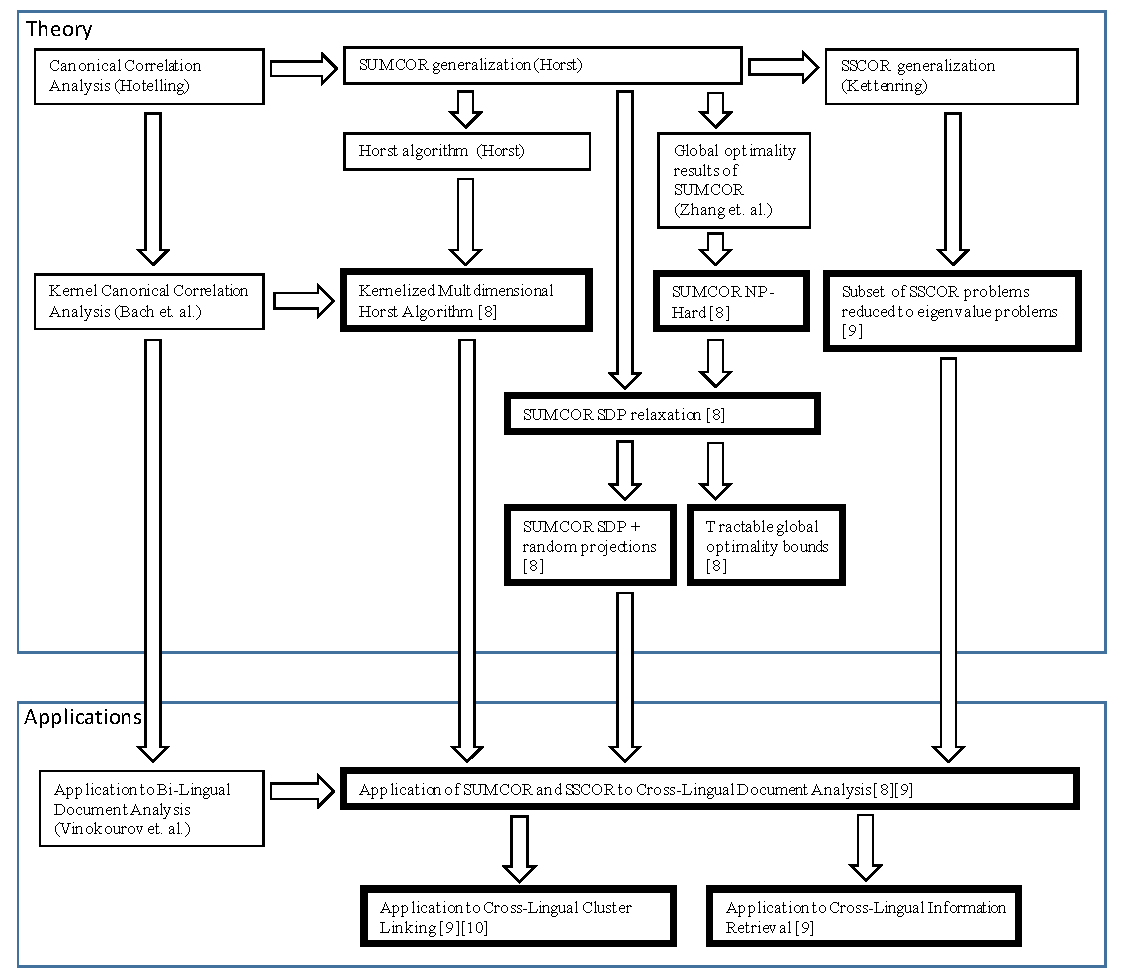
\includegraphics[width=1\textwidth]{figures/position_of_work.pdf}
\caption[The main contributions and related work]{The main contributions, represented by text boxes with thick border, are
positioned with respect to the related work.}
\label{fig:position_of_work}
\end{figure}

\section{Scientific Contributions}

We now list the main scientific contributions of the thesis and their references:
\begin{itemize}
\item A novel algorithm based on the Horst's algorithm that can extract several sets of nonlinear patterns ~\cite{DBLP:journals/corr/abs-1302-0974}
\item A proof that in general the Sum of Correlations problem is NP-hard ~\cite{DBLP:journals/corr/abs-1302-0974}
\item A semidefinite programming relaxation of the SUMCOR problem and
several new bounds on global optimization of the SUMCOR problems~\cite{DBLP:journals/corr/abs-1302-0974}
\item A novel approach to apply the SDP bounds on high-dimensional data~\cite{DBLP:journals/corr/abs-1302-0974}
\item A novel approach to building cross-lingual similarity functions and its application to cross-lingual information retrieval and cross-lingual cluster linking~\cite{rupnikJAIR}\cite{Belyaeva201564}
\item Addressing the missing data problem, a novel reduction of a subset of SSCOR problems to eigenvalue problems~\cite{rupnikJAIR}
\end{itemize}

\section{Thesis Structure}

The rest of the thesis is structured as follows. Chapter~\ref{chap:notation} introduces notation and some
definitions. For background we describe three pattern analysis methods that are the most relevant
for the thesis and explain how they can be adapted for analysis of nonlinear patterns in Chapter~\ref{chap:background}. Chapter~\ref{chap:extensions}
introduces a central problem of the thesis: generalizations of Canonical Correlation Analysis (CCA) and the original
contributions that extend the method to nonlinear and higher-dimensional setting. In Chapter~\ref{chap:relaxations}
we prove the result on the complexity of a particular generalization and study global optimality guarantees based
on semidefinite relaxations. Chapter~\ref{chap:crosslingual} discusses an application of multiview learning
to building cross-lingual similarity models. We show how a particular structure of the data can be exploited
to express a particular generalization of CCA as an eigenvector problem. Chapter~\ref{chap:applications} then
shows how the cross-lingual similarity measures can be used to perform cross-lingual cluster linking, relevant
for large scale monitoring of global news in multiple languages. In Chapter~\ref{chap:experiments} several experiments
are presented both on synthetic and real datasets. Finally, Chapter~\ref{chap:conclusions} concludes the thesis
and discusses possible future directions. 
%
% If needed, the thesis can consist of parts (not encouraged)
%\part{First Part of the Thesis}
%
% Second chapter 
%--------------------------------------------------------------------------------------------------
%
\chapter{Background}
%--------------------------------------------------------------------------------------------------

The central subjects in the thesis revolve around statistical approaches to finding structure in one, two or more sets of variates. We will
introduce two methods that find structure in a single set of variates: $k$-means clustering and Principal Component Analysis. We will then present
Canonical Correlation Analysis (CCA), a method for studying two sets of variates. We will also briefly cover kernel method extensions of the methods.


\section{$k$-means}\label{sec:kmeans}

The $k$-means algorithm is perhaps the most well-known and widely-used clustering algorithm. Here, we present its application
to compute cross-lingual similarities. The idea is based on concatenating the corpus matrices, running standard $k$-means clustering to obtain the matrix of centroids, ``reversing" the concatenation step to obtain a set of aligned bases, which are finally used to compute cross-lingual similarities. See Figure~\ref{fig:kmeans} for overview of the procedure. The left side of Figure~\ref{fig:kmeans} illustrates the decomposition and the right side summarizes the coordinate change.

\section{Cross-Lingual Latent Semantic Indexing}\label{sec:LSI}

The second approach we consider is Cross-Lingual Latent Semantic Indexing (CL-LSI)~\cite{cl_lsi} which is a variant of LSI~\cite{lsi} for more than one language. The approach is very similar to $k$-means, where we first concatenate the corpus matrices, compute a decomposition, which in case of CL-LSI is a truncated Singular Value Decomposition (SVD), decouple the
 column space matrix and use the blocks to compute linear maps to a common vector space, where standard cosine similarity is used to compare documents.

 The method is based on computing a truncated singular value decomposition of the concatenated corpus matrix $X \approx U S V^T$. See Figure~\ref{fig:lsi} for the decomposition. Representing documents in ``topic`` coordinates is done in the same way as in the $k$-means case (see Figure~\ref{fig:kmeans}), we will describe how to compute the coordinate change functions.

\begin{figure}[tbp]
\centering
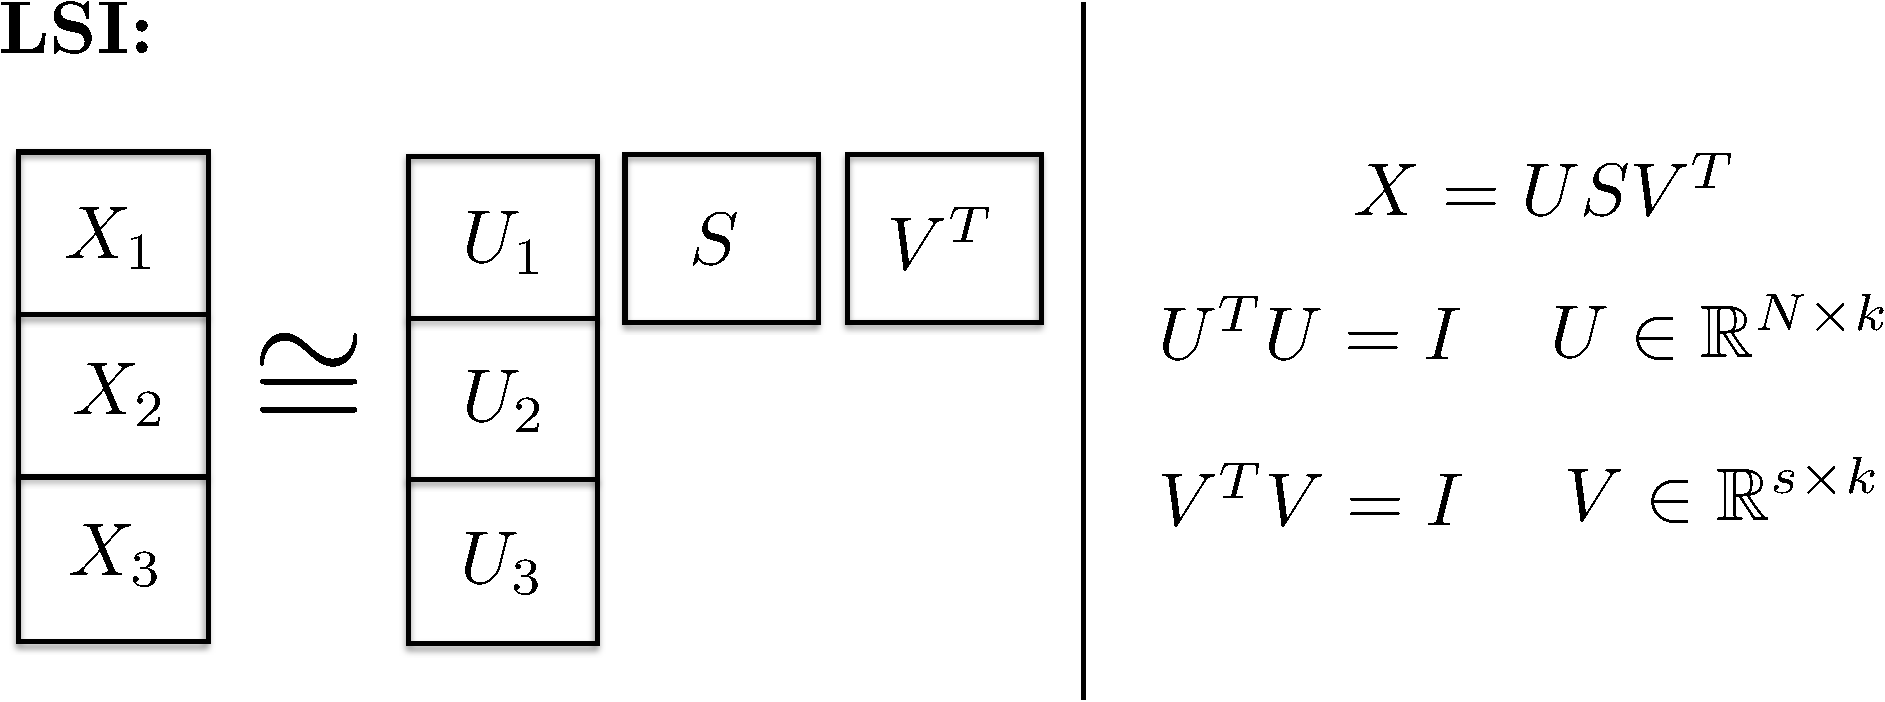
\includegraphics[width=10cm]{figures/lsi.pdf}
\caption{\label{fig:lsi} LSI multilingual corpus matrix decomposition.}
\end{figure}

The cross-lingual similarity functions are based on a rank-$k$ truncated SVD: $X \approx U \Sigma V^T,$ where $U \in \RR^{N \times k}$ are basis vectors of interest and $\Sigma \in \RR^{k \times k}$ is a truncated diagonal matrix of singular eigenvalues. An aligned basis is obtained by first splitting $U$ vertically according to the number of dimensions of each language: $U = [U_1^T \cdots U_m^T]^T$. Then, the same as with $k$-means clustering, we compute the pseudoinverses $P_i = (U_i^T U_i)^{-1} U_i^T$. The matrices $P_i$ are used to change the basis from the standard basis in $\RR^{n_i}$ to the basis spanned by the columns of $U_i$.

\paragraph{Implementation note}

  Since the matrix $X$ can be large we could use an iterative method like the Lanczos algorithm with reorthogonalization~\cite{golub} to find the left singular vectors (columns of $U$) corresponding to the largest singular values. It turns out that the Lanczos method converges slowly as the gap between the leading singular values is small. Moreover, the Lanczos method is hard to parallelize. Instead, we use a randomized version of the SVD~\cite{tropp} that can be viewed as a block Lanczos method. That enables us to use parallelization and speeds up the computation considerably.

To compute the matrices $P_i$ we used the QR algorithm~\cite{golub} to factorize $U_i$ as $U_i = Q_i R_i$, where $Q_i^TQ_i = I$ and $R_i$ is a triangular matrix. $P_i$ is then obtained by solving $R_i P_i = Q_i$.


\section{Canonical Correlation Analysis}

Canonical Correlation Analysis (CCA) ~\cite{Hotelling} is a general procedure for studying relationships between two sets of random variables. It is based on analyzing the cross-covariance matrix between two random vectors with the aim of identifying linear relationships between them. We will start with intuitions and then give a formal presentation.

Roughly speaking, given two random vectors $\mathcal{X}$ and $\mathcal{Y}$ we are interested in "non-trivial" pairs of functions $(f,g)$ such that there is a "dependence" between $f(\mathcal{X})$ and $g(\mathcal{Y})$. The "dependence" we consider is linear (possibly in a Hilbert space). The "non-triviality" of the functions is a requirement that guards us against trivial solutions, such as $f(x) := 0 \cdot x$, $g(y) := 0 \cdot y$ - that is, $f(\mathcal{X})$ and $\mathcal{X}$ should share some information, and analogously for $g(\mathcal{Y})$ and $\mathcal{Y}$. In other words, $f$ and $g$ should not destroy the original signals. When we are interested in more than one good pair of functions, for instance, a family of pairs $(f_i,g_i)$, we typically require additional constraints to prevent non-trivial solutions by enforcing that $f_i\left(\mathcal{X}\right)$ and $f_{j \neq i}\left(\mathcal{X}\right)$ share no information, and similarly for $g_i$. We are interested in essentially different function pairs.

There are several possible applications of such an analysis. For example, a common scenario involves analyzing objects $o \in \mathcal{O}$, where $\mathcal{O}$ is some underlying space, which are not directly observable, but are only observable as images of transformations $F: \mathcal{O} \rightarrow \RR^p$ and $G: \mathcal{O} \rightarrow \RR^q$. That is, we do not have access to $o$ but only to $\left(F(o), G(o)\right)$. Then finding function pairs $(f_i, g_i)$ so that $f_i(F(o))$ behave similarly as $g_i(G(o))$ can be interpreted as finding coupled parametrizations of image spaces of $F$ and $G$ which agree on $\mathcal{O}$. This enables applications such as cross-modal information retrieval, classification, clustering, etc. If $F$ encodes a visual image and $G$ encodes a textual description of the scene, we can perform text input based search over a collection of images, see~\cite{HardoonSS04}. Bi-lingual document analysis is another application, see~\cite{mrpqr}. The pattern functions $(f_i, g_i)$ themselves can be interesting to study for exploratory purposes.

Formally, let
$$ S = \{ \left( F(o_1), G(o_1) \right), \ldots, \left( F(o_n), G(o_n) \right) \} $$
represent a sample of $n$ pairs drawn independently at random according to the underlying distribution, where $F(x_i) \in \RR^p$ and $G(x_i) \in \RR^q$ represent feature vectors from $p$ and $q$-dimensional vector spaces. Let $X=[F(o_1), \ldots, F(o_n)]$ and let $Y=[G(o_1), \ldots ,G(o_n)]$ be the matrices with observation vectors as columns (using MATLAB notation).

The idea is to find two linear functionals (row vectors) $\alpha \in \RR^p$ and $\beta \in \RR^q$ so that the random variables $\alpha \cdot \mathcal{X}$ and $\beta \cdot \mathcal{Y}$ are maximally correlated ($\alpha$ and $\beta$ map the random vectors to random variables, by computing weighted sums of vector components). By using the sample matrix notation $X$ and $Y$ this problem can be formulated as the following optimization problem:

\begin{equation*}
\begin{aligned}
& \underset{\alpha \in \RR^{p}, \beta \in \RR^{q}}{\text{maximize}}
& & \frac{\alpha C_{XY} \beta'}{\sqrt{\alpha C_{XX} \alpha'} \sqrt{\beta C_{YY} \beta'}},
\end{aligned}
\end{equation*}
where $C_{XX}$ and $C_{YY}$ are empirical estimates of variances of $\mathcal{X}$ and $\mathcal{Y}$ respectively and $C_{XY}$ is an estimate for the covariance matrix. Assuming that the observation vectors are centered, the matrices are computed in the following way: $C_{XX} = \frac{1}{n-1}X X'$, $C_{YY} = \frac{1}{n-1}Y Y'$ and $C_{XY} = \frac{1}{n-1}X Y'$.
The optimization problem can be reduced to an eigenvalue problem and includes inverting the variance matrices $C_{XX}$ and $C_{YY}$. If the matrices are not invertible, one can use a regularization technique by replacing $C_{XX}$ with $(1- \kappa)C_{XX} + \kappa I$, where $\kappa \in [0,1]$ is the regularization coefficient and $I$ is the identity matrix.
A single canonical variable is usually inadequate in representing the original random vector and typically one looks for $k$ projection pairs $(\alpha_1, \beta_1),\ldots,(\alpha_k, \beta_k)$, so that $\alpha_i$ and $\beta_i$ are highly correlated and $\alpha_i$ is uncorrelated with $\alpha_j$  for $j \neq i$ and analogously for $\beta$.

The problem can be reformulated as a symmetric eigenvalue problem and solved efficiently. In case the dimensions of the problem $p$ and $q$ are large and observation vectors are sparse, one can consider an iterative method, for example Lanczos algorithm~\cite{LAL}). Alternatively, if the number of observation vectors $n$ is not prohibitively large, one can reformulate the problem to its dual representation which can be combined with a "kernel trick"~\cite{FBMJ} to yield nonlinear version of CCA.

A single canonical variable is usually inadequate in representing the original random vector and typically one looks for $k$ projection pairs $(w_i^1, w_j^1),\ldots,(w_i^k, w_j^k)$, so that $(w_i^{u})^T \mathcal{X}_i$ and $(w_j^{u})^T \mathcal{X}_j$ are highly correlated and $(w_i^{u})^T \mathcal{X}_i$ is uncorrelated with $(w_i^{v})^T \mathcal{X}_i$  for $u \neq v$ and analogously for $w_j^u$ vectors.


\section{Kernels and KCCA}

%
% Third chapter 
%--------------------------------------------------------------------------------------------------
%
\chapter{Extensions}
%--------------------------------------------------------------------------------------------------


\section{Introduction}
Natural phenomena are often the product of several factors
interacting. A fundamental challenge of pattern analysis and
machine learning is to find the relationships between these
factors. Real world datasets are often modeled using
distributions such as mixtures of Gaussians.  These models often
capture the uncertainty inherent in both underlying systems and
measurements. Canonical correlation analysis (CCA) is a
well-known and well-developed statistical technique developed to find the
relationships between two sets of random variables.
The relations or patterns discovered by CCA can be used
in two ways. First, they can be used to obtain a common representation for both sets of variables.
Second, the patterns themselves can be used in an exploratory analysis (e.g. see \cite{Hardoon_usingimage}).

It is possible to extend this idea beyond two sets. The
problem is then known as the Multi-set Canonical Correlation Analysis
(MCCA). Whereas it can be shown that CCA can be solved using an
(generalized) eigenvalue computation, MCCA is a much more
difficult problem. One approach is to express it as a
non-convex quadratically constrained quadratic program (QCQP). In
this paper, we show that despite being a highly structured
problem, it is NP-hard. We then describe an efficient algorithm
for finding a locally optimal solutions to the problem.

Since the algorithm is local and the problem non-convex, we
cannot guarantee the quality of the solutions
obtained. Therefore, we give a relaxation of the problem based on
semi-definite programming (SDP) which gives a constant factor
approximation as well as an output sensitive guarantee.

For use in practical applications, we describe two important
extensions: we adapt the methods to use kernels and to find
multi-dimensional solutions.

Finally, we perform extensive experimentation to compare the
efficient local algorithm and the SDP relaxation on both
synthetic and real-world datasets. Here, we show experimentally
that the hardness of the problem is in some sense generic in low
dimensions. That is, a randomly generated problem in low
dimensions will result in many local maxima which are far from
the global optimum. Somewhat surprisingly, this does not occur in
higher dimensions.%, where convergence to solutions that are not globally optimal is rare.

Our contributions in this paper are as follows:
\begin{itemize}
\item We show that in general MCCA is NP-hard.
\item We describe a scalable and efficient algorithm for finding a locally optimal solution.
\item Using an SDP relaxation of the problem, we can compute a
  global upper bound on the objective function along with various
  approximation guarantees on solutions based on this relaxation.
\item We describe two extensions which are important for practical applications: a kernel method and computing multiple sets of canonical vectors.
\item An extensive experimental evaluation of the respective algorithms: we show that in practice the local algorithm performs extremely well, something we can verify with using the SDP relaxation as well as show there are cases where the local algorithm is far from the optimal solution. We do this with a combination of synthetic and real world examples.
\item We propose a preprocessing step based on random projections, which enables us to apply the SDP bounds on large, high dimensional datasets.
\end{itemize}

\vspace{-0.1cm}
\section{Background}\label{sec:Background}
Canonical Correlation Analysis (CCA), introduced by Harold Hotelling \cite{Hotelling},  was developed to detect linear relations between two sets of variables. Typical uses of CCA include
statistical tests of dependence between two random vectors, exploratory analysis on multi-view data, dimensionality reduction and finding a common embedding of two random vectors that share mutual information.

 CCA has been generalized in two directions: extending the method to finding nonlinear relations  by using kernel methods \cite{FBMJ}\cite{HardoonCCA} (see \cite{shawe-taylor04kernel} for an introduction to kernel methods) and extending the method to more than two sets of variables which was introduced in \cite{Kettenring}. Among several proposed generalizations in \cite{Kettenring} the most notable is the sum of correlations (SUMCOR) generalization and it is the focus of our paper. There the goal is to project $m$ sets of random variables to $m$ univariate random variables, which are pair-wise highly correlated on average\footnote{Given $m$ univariate random variables, one can compute $\binom{m}{2}$ correlation coefficients, one for each pair of variables.}. An iterative method to solve the SUMCOR generalization was proposed in \cite{Horst} and the proof of convergence was established in \cite{Chu}. In \cite{Chu} it was shown that a generic SUMCOR problem admits exponentially many locally optimal solutions.
 In \cite{GlobalMEP2} the authors identified a subset of SUMCOR problems for which the iterative procedure converges to a global maximizer (Their results apply to nonnegative irreducible quadratic forms).
In our paper we show that easily computable necessary and sufficient global optimality conditions are theoretically impossible (which follows from the NP-hardness of the problem). Since in
practice good local solutions can be obtained we will present some results on sufficient global optimality.

We also focus on extensions of the local iterative approach \cite{Horst} to make the method practical. Here we show how the method can be extended to finding non-linear patterns and finding more than one set of canonical variates. Our work is related to \cite{JointBSSAppl} where a deflation scheme is used together with the Newton method to find several sets of canonical variates. Our nonlinear generalization is related to \cite{nonlinJointBSS}, where the main difference lies in the fact that we "kernelized" the problem, whereas the authors in \cite{nonlinJointBSS} worked with explicit nonlinear feature representation.

We now list some applications of the SUMCOR formulation. In \cite{kernelHyperAppl} an optimization problem for multi-subject functional magnetic resonance imaging (fMRI) alignment is proposed, which can be formulated as a SUMCOR problem (performing whitening on each set of variables). Another application of the SUMCOR formulation can be found in \cite{JointBSSAppl}, where it is used for group blind source separation on fMRI data from multiple subjects. An optimization problem equivalent to SUMCOR also arises in control theory \cite{ControlApplication} in the form of linear sensitivity analysis of systems of differential equations.
\vspace{-0.1cm}
\section{Sum of Correlations}\label{sec:sumcor}
\paragraph{Notation}
We first introduce the notation we use throughout the paper:
\begin{itemize}
\item Column vectors are denoted by lowercase
letters, e.g. $x$ and matrices are denoted by uppercase letters,
e.g. $X$.
\item Subscripts are used to
enumerate vectors or matrices, e.g. $x_1, x_2$, $X_1$, except in the
special case of the identity matrix, $I_n$ and the zero matrix $0_{k,l}$.
In these cases, the subscripts
denote row and column dimensions.
\item We use MATLAB notation (\cite{golub})% for vector and matrix transpose ($x^T$),
for referring to vector components (e.g. $x(i)$) , matrix elements, rows and columns {(e.g. ${X(i,j), X(i,:), X(:,j)}$)} and vector and matrix concatenation (e.g. $[A B]$).
\item Let $\RR^n$ denote the
$n$-dimensional
real vector space %and $\RR^{n\times m}$ denote
%the $(n \cdot m)$-dimensional vector space used when specifying
%matrix dimensions and let
 %$\NN$ denote the natural numbers and %. Furthermore, let
 and $\sym_n^{+}$ denote the space of symmetric positive definite $n$-by-$n$ matrices.
%\item Let $\norm{v}$ or $\norm{v}_2$ denote the $\ell_2$ norm of the vector $v$ and $\norm{A}_F$, $\norm{A}_1$ and $\norm{A}_2$ to denote the Frobenious norm and 1 and 2 matrix norms.% two commonly used operator norms of matrix $A$.
\end{itemize}
\vspace{-0.1cm}

Before defining  the problem formally, we  give some context and intuition.  Assume we have a random vector $\mathcal{X}$
distributed over $\RR^N$. Without loss of generality, assume it is
centered: $E\left(\mathcal{X}\right) = 0$ and let
$C$ denote the covariance matrix  $Cov\left(\mathcal{X}, \mathcal{X}\right)$. %of $\mathcal{X}$.


\noindent\textbf{Sum of Correlations.}
Canonical Correlation Analysis (CCA) is a method for analyzing two sets of random variables. The goal of CCA is
to identify one-dimensional projections of the two sets of variables that are maximally correlated. We study a generalization with more than two sets of variables.
The key aspect of this problem, which will repeatedly appear, is that we fix number of sets of variables. This assumes that $C$
has a \emph{block structure}. Informally, each block component of $\mathcal{X}$  is a \emph{view} of $\mathcal{X}$, where the views share some mutual information. The problem is to identify the one-dimensional projections of each view that maximize the average correlations across views.
%
%Throughout the paper we will use the block matrix and vector notation.
Let $m$ denote the number of blocks and  $N$ the total number of
elements. Then
$$b := \left(n_1, \ldots, n_m\right), \sum_{i=1}^m b\left(i\right) =
N$$
denotes the number
of elements in each of the blocks. We denote the corresponding
sub-vectors %according to the block structure $b$ are denoted
as $\mathcal{X}^{(i)} \in \RR^{n_i}$
($i$-th block-row of vector $\mathcal{X}$) and the sub-matrices as $C^{(i,j)} \in \RR^{n_i \times n_j}$ ($i$-th block-row, $j$-th block column of matrix $C$); see Figure~\ref{fig:block_structure}. For example, in CCA, there are only two sets, so $m=2$.
\begin{figure}[t]
\centering
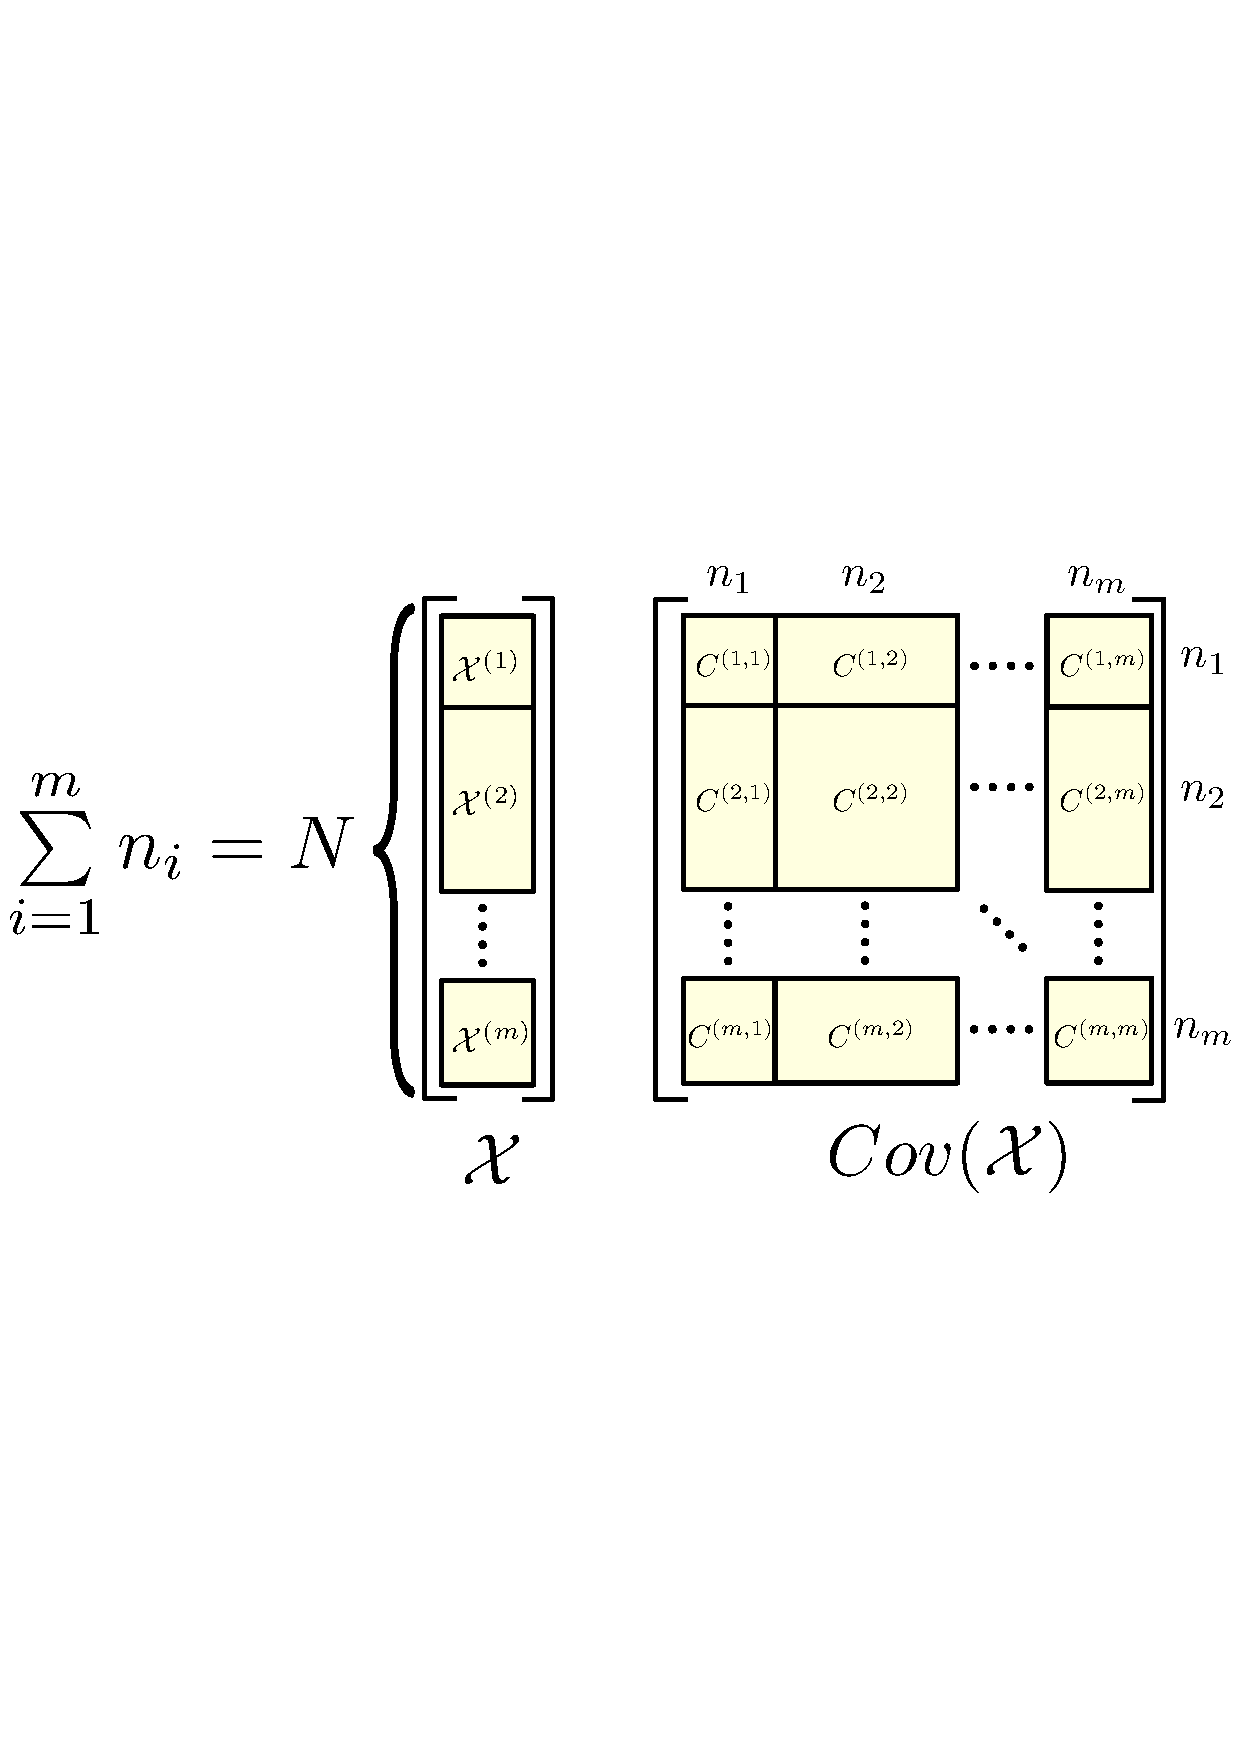
\includegraphics[width=0.5\textwidth]{figures/block_structure.pdf}
\caption{\label{fig:block_structure} The block structure of the  random vector $\mathcal{X}$ and the corresponding covariance block structure.}
\end{figure}
%
%

Formally, given $w \in \RR^N$ we define $m$ random variables $\mathcal{Z}_i$ (one-dimensional projections of random block components of $\mathcal{X}$) as:
\begin{equation*}
\mathcal{Z}_i := \sum_{j = 1}^{n_i} \mathcal{X}^{(i)}\left(j\right)
w^{(i)}\left(j\right) = \mathcal{X}^{(i)T} \cdot w^{(i)}.
\end{equation*}
%$\mathcal{Z}_i$ is a random variable computed as a linear combination of components of $\mathcal{X}^{(i)}$.
%
Let $\rho\left(x,y\right)$ denote the correlation
 coefficient between two random variables:
\begin{equation*}
\rho\left(x,y\right) =
 \frac{Cov\left(x,y\right)}{\sqrt{Cov\left(x,x\right) Cov\left(y,y\right)}}.
\end{equation*}
 The correlation coefficient between $\mathcal{Z}_i$ and
 $\mathcal{Z}_j$ can be expressed as:
\begin{equation*}
\rho\left(\mathcal{Z}_i, \mathcal{Z}_j\right) = \frac{w^{(i)T} C^{(i,j)}
   w^{(j)}}{\sqrt{w^{(i)T} C^{(i,i)} w^{(i)}}\sqrt{w^{(j)T}
     C^{(j,j)} w^{(j)}} }.
\end{equation*}
%
%
The problem described above can be stated as
finding the set of vectors $w^{(i)}$
which maximize
\begin{equation}\label{eq:SUMCOR}
\tag{SUMCOR}
\sum_{i = 1}^m \sum_{j = i+1}^m
\rho\left(\mathcal{Z}_i, \mathcal{Z}_j\right).
\end{equation}
We refer to this problem as Multi-set Canonical
Correlation Analysis (MCCA). Note that it reduces to CCA when
$m=2$. The solution - that is, the set of components $\left(w^{(1)}, \ldots, w^{(m)}\right)$, are referred to as the set of canonical vectors.% We refer to each
%$\mathcal{X}^{(i)}$ as a particular view of some underlying
%object where the assumption is that random vectors
%$\mathcal{X}^{(i)}$ share some mutual information (i.e. are not independent).
%

\noindent\textbf{Reformulating the optimization problem.} Expanding SUMCOR,
we get:
\begin{equation*}
\begin{aligned}
& \underset{w \in \RR^N}{\text{max}} & & \sum_{i = 1}^m
  \sum_{j = i+1}^m \frac{w^{(i)T} C^{(i,j)}
    w^{(j)}}{\sqrt{w^{(i)T} C^{(i,i)} w^{(i)}} \sqrt{w^{(j)T}
      C^{(j,j)} w^{(j)}}}.
\end{aligned}
\end{equation*}
%
%%some explanation
%
Observe that the solution is invariant to scaling (only the direction matters): if $\left(w^{(1)}, \ldots, w^{(m)}\right)$ is a solution, then $\left(\alpha_1 \cdot w^{(1)}, \ldots, \alpha_m \cdot w^{(m)}\right)$ is also a solution for $\alpha_i > 0$. We may therefore impose constraints $w^{(i)T}C^{(i,i)}w^{(i)} = 1$, which only affect the norm. This yields the following
 equivalent constrained problem:
\begin{equation}\label{eq:qcqp0}
\begin{aligned}
& \underset{w \in \RR^N}{\text{maximize}}
& & \sum_{i = 1}^m \sum_{j = i+1}^m w^{(i)T} C^{(i,j)} w^{(j)}\\
& \text{subject to}
& &w^{(i)T} C^{(i,i)} w^{(i)} = 1, \quad\forall i = 1,\ldots, m.
\end{aligned}
\end{equation}
%
We further multiply the objective by $2$ and add a constant $m$. Note that this does not
affect the optimal solution. Using the equalities: $w^{(i)T} C^{(i,j)} w^{(j)} = w^{(j)T} C^{(j,i)} w^{(i)}$ and $w^{(i)T} C^{(i,i)} w^{(i)} = 1$, we obtain:
%
%
\begin{equation}\label{eq:qcqp05}
\begin{aligned}
& \underset{w \in \RR^N}{\text{maximize}}
& & \sum_{i = 1}^m \sum_{j = 1}^m w^{(i)T} C^{(i,j)} w^{(j)}\\
& \text{subject to}
& &w^{(i)T} C^{(i,i)} w^{(i)} = 1, \quad\forall i = 1,\ldots, m.
\end{aligned}
\end{equation}
This transforms the objective function into a quadratic form $w^T C w$. To
simplify the constraints, assume that $C^{(i,i)}$ is strictly positive definite. If $C^{(i,i)}$ is not full rank, then using the eigenvalue decomposition $C^{(i,i)} = V \Lambda V^T$, where $V \in \RR^{n_i \times k}$, $\Lambda \in \RR^{n_i \times k}$, $\Lambda > 0$, $k < n_i$, we substitute $\mathcal{X}^{(i)}$ with $V^T \mathcal{X}^{(i)} \in \RR^k$, for which the covariance matrix is strictly positive definite.
%
%
From the strict positive definiteness it follows that $C^{(i,i)}$ admits a Cholesky decomposition: there exists an invertible matrix $D_i$ such that $C^{(i,i)} = D_i^T D_i$.

Finally, using the block structure $b$, we substitute $w^{(i)}$ with $D_i^{-1} x^{(i)}$ and define $A \in \RR^N$ as:
\begin{equation*}
A^{(i,j)} := {D_i}^{-T} C^{(i,j)} {D_j}^{-1},
\end{equation*}
leading to the simplified problem:
 \begin{equation}\label{eq:qcqp}
\tag{QCQP}
\begin{aligned}
& \underset{x \in \RR^{N}}{\text{max}}
& & x^T A x\\
& \text{subject to}
& &x^{(i)T} x^{(i)} = 1, \quad\forall i = 1, \ldots, m.
\end{aligned}
\end{equation}
It turns out that (\ref{eq:qcqp}) is simpler to  manipulate than  (\ref{eq:SUMCOR}), so we use this form from this point on.





\vspace{-0.1cm}
\section{Extensions}\label{sec:sumcorextensions}
Here we present two extensions of MCCA: how to use kernel methods with
MCCA to find nonlinear dependencies in the data; and an
algorithm to finding more then one set of correlation vectors.
\subsection{Dual representation and kernels}\label{subsec:kernels}
%\label{sect:primal}
We return to formulation (\ref{eq:qcqp0}):
 \begin{equation*}
\begin{aligned}
& \underset{w \in \RR^N}{\text{max}}
& & \sum_{i = 1}^m \sum_{j = i+1 }^m w^{(i)T} C^{(i,j)} w^{(j)}\\
& \text{subject to}
& &w^{(i)T} C^{(i,i)} w^{(i)} = 1, \quad\forall i = 1,\ldots, m,
\end{aligned}
\end{equation*}
  where $b = \left(n_1,\ldots,n_m\right)$ denotes the block structure
  and $ \sum_i n_i = N $.
 In the previous sections, we focused on manipulating covariance matrices only and omitted details on their estimation based on finite samples. In this section, we will use a formulation that explicitly presents the empirical estimates of covariances, which will enable us to apply kernel methods.
Let $\mathcal{X}$ be a random vector distributed over $\RR^N$ with
$E\left(\mathcal{X}\right) = 0$. Let $X \in \RR^{N \times s}$
represent a sample of $s$ observations of $\mathcal{X}$, where each
observation corresponds to a column vector. The empirical covariance of $\mathcal{X}$ based on the sample matrix $X$ is expressed as: $$ \overline{Cov\left(\mathcal{X}\right)} = \frac{1}{s - 1}X X^T.$$
If $s < N$, then $\overline{Cov\left(\mathcal{X}\right)}$ is singular which makes the optimization problem ill-posed and may lead to overfitting (discovering spurious patterns in the data). These issues are addressed by using regularization techniques, typically a shrinkage estimator $\overline{Cov\left(\mathcal{X}\right)_{\kappa}}$ is defined as: $$ \overline{Cov\left(\mathcal{X}\right)_{\kappa}} = \left(1-\kappa\right) \frac{1}{s - 1}X X^T + \kappa  I_N,$$ where $\kappa \in \left[0,1\right]$.

Using the block structure $b$, (\ref{eq:qcqp05}) becomes:
 \begin{equation}\label{eq:regqcqp}
\begin{aligned}
& \underset{w \in \RR^N}{\text{max}}
& & \frac{1}{s -1} \sum_{i = 1}^m \sum_{j = i+1}^m w^{(i)T} X^{(i)}X^{(j)T} w^{(j)} \\
& \text{subject to}
& & w^{(i)T} \left(\frac{1- \kappa}{s - 1}X^{(i)} X^{(i)T} + \kappa  I_N\right) w^{(i)} = 1,\\&&& \quad\forall i = 1,\ldots, m.
\end{aligned}
\end{equation}
To express each component $w^{(i)}$ in terms the columns of $X^{(i)}$,
let $w$ have block structure $b_w = \left(n_1, \ldots, n_m\right)$
where $\sum_i n_i = N$, and let $y \in \RR^{m\cdot s}$ have block
structure $b_y\left(i\right) = s, \forall i = 1,\ldots, m$. The
component $w^{(i)}$ can be expressed as:
\begin{equation}\label{eq:representer}
\begin{aligned}
w^{(i)} = \sum_{j = 1}^{s} y^{(i)}\left(j\right) X^{(i)}\left(:,j\right) = X^{(i)} y^{(i)}.
\end{aligned}
\end{equation}
We refer to $y$ as dual variables.
%
%
%It remains to check that the formulations (\ref{eq:regqcqp}) and (\ref{eq:dualregqcqp}) are equivalent. We need to check that the optimal solution to (\ref{eq:regqcqp}) can be expressed by using dual variables \eqref{eq:representer}.
\begin{lemma}
There exists a solution to \eqref{eq:regqcqp} which can be expressed as \eqref{eq:representer}.
\end{lemma}
\begin{proof}
We prove the lemma by contradiction. Assume that no optimal solution
can be expressed as \eqref{eq:representer} and $u$ be an optimal solution to the problem \eqref{eq:regqcqp}. Without loss of generality, assume that $u^{(1)}$ does not lie in the column space of $X^{(1)}$:
 $$u^{(1)} = z_{\bot} + X^{(1)} y^{(1)},$$
 where
$$z_{\bot} \neq 0_{n_1}\quad \text{and}\quad X^{(1)T}z_{\bot} = 0_s.$$
We show that $\bar{u}$, defined as $\bar{u}^{(i)} := u^{(i)}, \forall i> 1$ and $\bar{u}^{(1)} := \frac{1}{\gamma}  X^{(1)} y^{(1)},$ where
\begin{equation*}
\gamma :=\sqrt{ y^{(1)T} X^{(1)T} \left(\frac{1- \kappa}{s - 1}X^{(1)} X^{(1)T} + \kappa  I_N\right) X^{(1)} y^{(1)} },
\end{equation*}
strictly increases the objective function, which contradicts the assumption that $u$ is optimal. Clearly, $\bar{u}$ is a feasible solution. Positive definiteness of $\frac{1- \kappa}{s - 1}X^{(1)} X^{(1)T} + \kappa  I_N$, coupled with the fact that $z_{\bot}^T z_{\bot} > 0$ implies that $0 < \gamma < 1$. Let $E := \sum_{j = 2}^m \left(X^{(1)} y^{(1)}\right)^T X^{(1)}X^{(j)T} u^{(j)}$.
%
If $E < 0$, then the
vector $[-u^{(1)T} u^{(2)T} \cdots u^{(m)T}]^T$ strictly increases the
objective function, which is a contradiction. We also obtain a contradiction if $E = 0$, since any nonzero $v \in \RR^{s}$ for which $X^{(1)}v \neq 0_{n_1}$ can be used to obtain a solution to the problem \eqref{eq:regqcqp} expressed as \eqref{eq:representer} (after re-scaling  such that $\overline{Cov\left(\mathcal{X}^{(1)}v\right)_\kappa} = 1$ and if necessary multiplying it by $-1$ so that $\sum_{j = 2}^m \left(X^{(1)} v\right)^T X^{(1)}X^{(j)T} u^{(j)}) \geq 0$).
Thus, we may assume that $E > 0$.
%If the sum was zero, then any properly scaled (with proper sign) combination of the training data $X^{(1)}$ could be used in place of $u^{(1)}$).
%
The following inequality completes the proof, since it shows that $\bar{u}$ increases the objective function:
%Note that $\frac{1}{s -1}  u^{(i)T} X^{(i)}X^{(j)T} u^{(j)} = \frac{1}{s -1}  \bar{u}^{(i)T} X^{(i)}X^{(j)T} \bar{u}^{(j)}$ where $i > 1$ and $j > 1$ and $u^{(1)T} (\frac{1- \kappa}{s - 1}X^{(1)} X^{(1)T} + \kappa  I_N) u^{(1)} = \bar{u}^{(1)T} (\frac{1- \kappa}{s - 1}X^{(1)} X^{(1)T} + \kappa  I_N) \bar{u}^{(1)} = 1$.
\begin{align*}
  \frac{1}{s -1} & \sum_{j = 2}^m u^{(1)T} X^{(1)}X^{(j)T} u^{(j)} =\\
= \frac{1}{s -1} & \sum_{j = 2}^m \left(z_{\bot} + X^{(1)} y^{(1)}\right)^T X^{(1)}X^{(j)T} u^{(j)} = \\
= \frac{1}{s -1}  &\sum_{j = 2}^m \left(X^{(1)} y^{(1)}\right)^T X^{(1)}X^{(j)T} u^{(j)} < \\
< \frac{1}{s -1}  &\sum_{j = 2}^m \frac{1}{\gamma}\left(X^{(1)} y^{(1)}\right)^T X^{(1)}X^{(j)T} u^{(j)}.
\end{align*}
%\qed
\end{proof}


%\substack{j = 1\\ j\neq i}

Let $K_i = X^{(i)T} X^{(i)} \in \RR^{s \times s}$ denote the Gram
matrix. Next, we express the problem (\ref{eq:regqcqp}) in terms of the dual variables:
 \begin{equation}\label{eq:dualregqcqp}
\begin{aligned}
& \underset{y \in \RR^{m\cdot s}}{\text{max}}
& & \frac{1}{s -1} \sum_{i = 1}^m \sum_{j = i+1}^m y^{(i)T} K_i K_j^T y^{(j)} \\% + \sum_{i = 1}^m y^{(i)T} (\frac{1 - \kappa}{s - 1}K_i  K_i^T + \kappa  K_i) y^{(i)}\\
& \text{subject to}
& & y^{(i)T} \left(\frac{1- \kappa}{s - 1}K_i K_i^T + \kappa  K_i\right) y^{(i)} = 1,\\
& &&\quad\forall i = 1,\ldots, m.
\end{aligned}
\end{equation}
Expressing the problem in terms of Gram matrices makes it amenable to using kernel methods (see \cite{shawe-taylor04kernel}).% which
%enable discovering nonlinear patterns in the data.


Typically the matrices $K_i$ are ill conditioned (or even singular
when the data is centered) and it is advantageous to constrain the
magnitude of dual coefficients as well as the variance in the original
problem. We address this by introducing a first order approximation to
the dual regularized variance.  Let $$\widetilde{K_i} :=
\left(\sqrt{\frac{1-\kappa}{s - 1}}K_i + \frac{\kappa}{2}
  \sqrt{\frac{s-1}{1- \kappa}}I_s\right).$$ The covariance becomes:
%
 $$ \overline{Cov\left(\mathcal{X}^{(i)}\right)_{\kappa}} =  \frac{1- \kappa}{s - 1}K_i K_i^T + \kappa  K_i \approx  \widetilde{K_i} \widetilde{K_i}^T.$$
This approximation has two advantages: it is invertible and is in a
factorized form. We exploit the latter when obtaining a convergent local method.
The final optimization is then expressed as:
 \begin{equation}\label{eq:approxdualqcqp}
\begin{aligned}
& \underset{y \in \RR^{m\cdot s}}{\text{max}}
& & \frac{1}{s -1} \sum_{i = 1}^m \sum_{j = i+1}^m y^{(i)T} K_i K_j^T y^{(j)}\\% + \sum_{i = 1}^m y^{(i)T} \widetilde{K_i} \widetilde{K_i}^T y^{(i)}\\
& \text{subject to}
& & y^{(i)T} \widetilde{K_i} \widetilde{K_i}^T y^{(i)} = 1, \quad\forall i = 1,\ldots, m.
\end{aligned}
\end{equation}
%
The problem can be interpreted as maximizing covariance while constraining variance and magnitude of dual coefficients. %Notice that the sum in the objective $\sum_{i = 1}^m y^{(i)T} \widetilde{K_i} \widetilde{K_i}^T y^{(i)}$ is constant and thus redundant. It is useful to keep it in order to obtain a reformulation of the problem where the local method provably converges.

%\subsection{Regularization}
%To prevent overfitting and make the problem numerically stable (as in CCA) we propose a regularization scheme. Let $\kappa \in [0,1]$ and let $\tilde{K}_i := (1-\kappa)K_i + \kappa I$, solve:
%\begin{equation}\label{equation:regdual}\max_{\beta_1, \ldots, \beta_m} \sum_{i < j} \beta_i' K_i K_j \beta_j,\end{equation} s.t. $$\beta_i'\tilde{K}_i \tilde{K}_i \beta_i = 1, \quad \forall i.$$
%The main benefit of this form of regularization is the a priori Cholesky-like decomposition (the factors are not triangular). This form of regularization is provably equivalent to regularization in \cite{FBMJ}.


\subsection{Computing several sets of canonical vectors}\label{subsec:severalCanonicalVectors}
Usually a one-dimensional representation does not sufficiently capture
all the information in the data and higher dimensional subspaces are
needed. After computing the first set of primal canonical vectors we
proceed to computing the next set. The next set should be almost as
highly correlated as the first one, but essentially ``different'' from
the first one. We achieve this by imposing additional constraints for
every view. Namely, all projection vectors in view $i$ are
uncorrelated with respect to $\widetilde{K}_i^2$ (this is similar to
the approach in two view regularized kernel CCA\cite{FBMJ}).
\par
Let $Y = \left[y_1, \ldots, y_k\right] \in \RR^{m\cdot s  \times k}$ represent $k$ sets of canonical vectors, where
$$Y^{(\ell)T} \widetilde{K_{\ell}^2} Y^{(\ell)} = I_k  \quad\forall \ell = 1,\ldots, m. $$
The equation above states that each canonical vector has unit regularized variance and that different canonical vectors corresponding to the same view are uncorrelated (orthogonal with respect to $\widetilde{K_i^2}$).


%%\delta_{ij} \forall \ell = 1,\ldots, m$$
%%where $$\delta_{ij}  = \left\{ \begin{array}{lll}
%%0 & {\rm for} ~i \neq j \\
%%1 & {\rm for} ~i = j   \end{array} \right.$$

%%_i = (y_i^1, \ldots, y_i^k)$ is the matrix
%%of $k$ uncorrelated vectors with respect to $\tilde{K}_i$, for every
%%view $i$. We are searching for the set of vectors $\beta_1^{k+1},
%%\ldots, \beta_m^{k+1}$ with unit regularized variance that maximize
%%the \textsc{sumcor} objective and are uncorrelated with the first $k$
%%solutions:
%%$${\beta_i^{k+1}}' \tilde{K}_i^2 \beta_i^{j}, \forall j < k+1, \forall i,$$
%%which can be written as:
%%$${\beta_i^{k+1}}'\tilde{K}_i^2 B_i = 0 , \forall i.$$

We will now extend the set of constraints in the optimization (\ref{eq:approxdualqcqp}) to enforce the orthogonality.
%
 \begin{equation}\label{eq:kdimapproxdualqcqp}
\begin{aligned}
& \underset{y \in \RR^{m\cdot s}}{\text{max}}
& & \frac{1}{s -1} \sum_{i = 1}^m \sum_{j = i+1}^m y^{(i)T} K_i K_j^T y^{(j)}\\% + \sum_{i = 1}^m y^{(i)T} \widetilde{K_i} \widetilde{K_i}^T y^{(i)}\\
& \text{subject to}
& & y^{(i)T} \widetilde{K_i} \widetilde{K_i}^T y^{(i)} = 1, \quad\forall i = 1,\ldots, m\\
& & & Y^{(i)T} \widetilde{K_i} \widetilde{K_i}^T y^{(i)} = 0_k, \quad\forall i = 1,\ldots, m.
\end{aligned}
\end{equation}
%
%
To use the Horst algorithm, we first use the substitutions:
$$Z^{(i)} = \widetilde{K_i}Y^{(i)}, \quad z^{(i)} = \widetilde{K_i}y^{(i)}$$
and define the operators $$P_i = I_s - \widetilde{K}_i Y^{(i)} Y^{(i)T} \widetilde{K}_i = I_s - Z^{(i)} Z^{(i)T},$$ which map to the space orthogonal to the columns of $\widetilde{K}_i Y^{(i)}$. Each $P_i$ is a projection operator: $P_i^2 = P_i,$ which follows directly from the identities above.
The optimization problem in the new variables is:
%
 \begin{equation}\label{eq:Zkdimapproxdualqcqp}
\begin{aligned}
& \underset{z \in \RR^{m\cdot s}}{\text{max}}
& & \frac{1}{s -1} \sum_{i = 1}^m \sum_{j = i+1}^m z^{(i)T} \widetilde{K_i}^{-T} K_i K_j^T \widetilde{K_j}^{-1} z^{(j)} \\%+ \sum_{i = 1}^m z^{(i)T} z^{(i)}\\
& \text{subject to}
& & z^{(i)T}  z^{(i)} = 1, \quad\forall i = 1,\ldots, m\\
& & & Z^{(i)T} z^{(i)} = 0_k, \quad\forall i = 1,\ldots, m.
\end{aligned}
\end{equation}
%
%
%
Using the projection operators, this is equivalent to:
\begin{equation*}%\label{eq:projZkdimapproxdualqcqp}
\begin{aligned}
& \underset{z \in \RR^{m\cdot s}}{\text{max}}
& & \frac{1}{s -1} \sum_{i = 1}^m \sum_{j = i+1}^m z^{(i)T} P_i^T \widetilde{K_i}^{-T} K_i K_j^T \widetilde{K_j}^{-1} P_j z^{(j)}\\% + \sum_{i = 1}^m z^{(i)T}  z^{(i)}\\
& \text{s.t.}
& & z^{(i)T}  z^{(i)} = 1, \quad\forall i = 1,\ldots, m.
\end{aligned}
\end{equation*}
%
By multiplying the objective by $2$ (due to the symmetries of $P_i, K_i$ and $\widetilde{K_i}$) and shifting the objective function by $\frac{m}{1 - \kappa}$, the problem is equivalent to:
\begin{equation}%\label{eq:projZkdimapproxdualqcqp}
\begin{aligned}
& \underset{z \in \RR^{m\cdot s}}{\text{max}}
& & \frac{1}{s -1} \sum_{i = 1}^m \sum_{\substack{j = 1\\ j\neq i}}^m z^{(i)T} P_i^T \widetilde{K_i}^{-T} K_i K_j^T \widetilde{K_j}^{-1} P_j z^{(j)}\\
&&& + \frac{1}{1-\kappa}\sum_{i = 1}^m z^{(i)T}  z^{(i)}\\
& \text{s.t.}
& & z^{(i)T}  z^{(i)} = 1, \quad\forall i = 1,\ldots, m.
\end{aligned}
\end{equation}
%
%
%
This optimization can be reformulated as:
\begin{equation}\label{eq:projZkdimapproxdualqcqp}
\begin{aligned}
& \underset{z \in \RR^{m\cdot s}}{\text{max}}
& & z^T A z\\
& \text{subject to}
& & z^{(i)T}  z^{(i)} = 1, \quad\forall i = 1,\ldots, m,
\end{aligned}
\end{equation}
where $A \in \RR^{m\cdot s}$ with block structure $b\left(i\right) = s, \forall i = 1,\ldots, m$, defined by:
\begin{equation*}
 A^{(i,j)} = \left\{ \begin{array}{lll}
 \frac{1}{s -1} P_i^T \widetilde{K_i}^{-T} K_i K_j^T \widetilde{K_j}^{-1} P_j  & {\rm for} ~i \neq j\\
\frac{1}{1-\kappa } I_s & {\rm for} ~i = j \end{array}\right\}.
\end{equation*}
%
\begin{lemma}
The block matrix $A$ defined above is positive semidefinite (i.e. $A \in \sym_+^{m\cdot s}$).
\end{lemma}
\begin{proof}
$A$ is symmetric, which follows from $P_i = P_i^T$ and $K_i =
K_i^T$. Let $z \in \RR^{m\cdot s}$.  The goal is to show that $z^T A z > 0$.
Let us define an auxiliary matrix $W$ as:
\begin{equation*}
\begin{aligned}
W =  \frac{1}{1- \kappa }&\sum_{i = 1}^m z^{(i)T} P_i^T
\widetilde{K_i}^{-T} \cdot \\&\left( \kappa K_i + \frac{\kappa^2
    \left(s-1\right)}{4\left(1-\kappa\right)}I_s   \right)
\widetilde{K_i}^{-1} P_i z^{(i)}
\end{aligned}
\end{equation*}
 Each summand is positive-semidefinite, i.e. $W \geq 0$ and $W > 0$ if $\exists i: P_i z^{(i)} = z^{(i)}$. What follows is a sequence of inequalities, some of which must
 be strict, as will be established:
\begin{align}
z^T A z &=  \frac{1}{s -1} \sum_{i = 1}^m \sum_{\substack{j = 1\\j\neq i}}^m z^{(i)T} P_i^T \widetilde{K_i}^{-T} K_i K_j^T \widetilde{K_j}^{-1} P_j z^{(j)}\nonumber
\\& \qquad + \frac{1}{1- \kappa }\sum_{i = 1}^m z^{(i)T}  z^{(i)} \label{proof_line_1}\\
%
&\geq \frac{1}{s -1} \sum_{i = 1}^m \sum_{\substack{j = 1\\ j\neq i}}^m z^{(i)T} P_i^T \widetilde{K_i}^{-T} K_i K_j^T \widetilde{K_j}^{-1} P_j z^{(j)}\nonumber\\
& \qquad + \frac{1}{1- \kappa }\sum_{i = 1}^m z^{(i)T} P_i^T P_i z^{(i)}  \label{proof_line_2}\\
%
 &= \frac{1}{s -1} \sum_{i = 1}^m \sum_{\substack{j = 1\\ j\neq i}}^m z^{(i)T} P_i^T \widetilde{K_i}^{-T} K_i K_j^T \widetilde{K_j}^{-1} P_j z^{(j)}\nonumber\\
 & \qquad+ \frac{1}{1- \kappa }\sum_{i = 1}^m z^{(i)T} P_i^T \widetilde{K_i}^{-T}  \widetilde{K_i}^T \widetilde{K_i} \widetilde{K_i}^{-1} P_i z^{(i)}  \label{proof_line_3}\\
%
&= \frac{1}{s -1} \sum_{i = 1}^m \sum_{\substack{j = 1\\ j\neq i}}^m z^{(i)T} P_i^T \widetilde{K_i}^{-T} K_i K_j^T \widetilde{K_j}^{-1} P_j z^{(j)}\nonumber
\\& \qquad+ \frac{1}{s-1}\sum_{i = 1}^m z^{(i)T} P_i^T \widetilde{K_i}^{-T}  K_i K_i^T \widetilde{K_i}^{-1} P_i z^{(i)} + W  \label{proof_line_4}\\
%+ \frac{1}{1- \kappa }&\sum_{i = 1}^m z^{(i)T} P_i^T \widetilde{K_i}^{-T} \left( \kappa K_i + \frac{\kappa^2 \left(s-1\right)}{4\left(1-\kappa\right)}I_s   \right) \widetilde{K_i}^{-1} P_i z^{(i)}
 &= z^T B B^T z + W \geq 0\nonumber,
\end{align}
where $B \in \RR^{m\cdot s \times s}$, defined by $B^{(i)} = \frac{1}{\sqrt{s-1}}(K_i \widetilde{K_i}^{-1}P_i)^T$, with corresponding row block structure $b\left(i\right) = s$. The inequality after (\ref{proof_line_1}) holds since projection operators cannot increase norms.
(\ref{proof_line_3}) is equal to (\ref{proof_line_2}) using $\widetilde{K_i}^{-T}  \widetilde{K_i}^T = I$.
Regrouping the terms and applying the definition of $W$, we obtain (\ref{proof_line_4}).
The final equality follows, since the first two sums form a perfect square.

Now we will show that at least one of the two inequalities is strict. If $P_i z^{(i)} \neq z^{(i)}$ for some $i$, then the first inequality is strict ($\norm{P_i z^{(i)}} < \norm{z^{(i)}}$). Conversely, if $P_i z^{(i)} = z^{(i)}$ for all $i$, then $W > 0$, hence the last inequality is strict.%\qed
\end{proof}



Matrix $A$ has all the required properties for convergence, so we
apply Algorithm \ref{algorithm:horst}. Solutions to
\eqref{eq:kdimapproxdualqcqp} are obtained by back-substituting into $y^{(i)} = \widetilde{K_i}^{-1} z^{(i)}$.


%%\begin{equation}\max_{y \in \RR^{m\cdot s}} \sum_{i < j} \beta_i' K_i K_j \beta_j   + \frac{1}{2(1-\kappa)^2}\sum_i \beta_i' \tilde{K}_i^2 \beta_i,\end{equation} s.t. $$\beta_i'\tilde{K}_i \tilde{K}_i \beta_i = 1, \quad \forall i$$\begin{equation}{B_i^k}' \tilde{K}_i^2 \beta_i = 0, \forall i.\end{equation}
%
%The solution to the above problem can be found by solving the following MEP:
%
%$$\sum_{j \neq i}P_i \tilde{K}_i^{-1} K_i K_j\tilde{K}_j^{-1} P_j
%\alpha_j + \frac{1}{(1-\kappa)^2}\alpha_i +  \lambda_i \alpha_i = 0,
%\forall i.$$
%
%followed by multiplying the solutions $\alpha_i$ by $\tilde{K}_i^{-1}$.
%
%Eigenvalue shifting techniques can be applied to force positive-definiteness (details omitted).
% The algorithm is
%shown in Algorithm \ref{fullalg}.
%

%\begin{algorithm}
%\caption{Horst algorithm for computing a $k$-dimensional representation}
%Input: $K_1, \ldots, K_m$, $\kappa$, $maxiter$, $k$, \par
%Output: $B_1^k, \ldots, B_m^k$
%\begin{algorithmic}
%\label{fullalg}
%\STATE $\tilde{K}_i = (1-\kappa) K_i +  \kappa I, \forall i$
%\FOR{$d = 1$ to $k$}
%\STATE Choose random vectors $\alpha_1^0, \ldots, \alpha_m^0$
%\IF{$d > 1$}
%\STATE $P_i^d =I -  \tilde{K}_i B_i^{d-1} {B_i^{d-1}}' \tilde{K}_i$
%\STATE Set $\alpha_i^0 \leftarrow P_i^d \alpha_i^0,~~~~ \forall i$
%\ELSE
%\STATE  $P_i^d = I ~~~~ \forall i$
%\ENDIF
%\STATE $u_i^0 = K_i \tilde{K}_i^{-1} \alpha_i^0, \forall i$
%\FOR{$i = 1$ to $maxiter$}
%\FOR{$j =1$ to $m$}
%\STATE $\alpha_j^{i} \leftarrow  P_j^d \tilde{K}_j^{-1} K_j \sum_{k\neq j}  u_k^{i-1}  + \left(\frac{1}{(1-\kappa)^2} \right) \alpha_j^{i-1}$
%\STATE $\alpha_j^{i} \leftarrow \frac{\alpha_j^{i}}{\sqrt{{\alpha_j^i}' \alpha_j^i}}$
%\STATE $u_j^{i} \leftarrow  K_k  \tilde{K}_k^{-1}  \alpha_k^{i}$
%\ENDFOR
%\ENDFOR
%\FOR{$l = 1$ to $m$}
%\STATE $\beta_l^d = \tilde{K}_l^{-1} \alpha_l^{maxiter}$
%\STATE $B_l^{d} = [ B_l^d , \beta_l^d]$ if $d > 1$
%\STATE $B_l^{d} = [ \beta_l^d]$ if $d = 1$
%\ENDFOR
%\ENDFOR
%\end{algorithmic}
%\end{algorithm}



\subsection{Implementation}\label{subsec:implementation}
The algorithm requires matrix vector multiplications and inverted
matrix vector multiplications. If the kernel matrices are products of
sparse matrices: $K_i = X^{(i)T} X^{(i)}$ with each $X^{(i)}$ having
$s\cdot n$ elements
where $s << n$, then the kernel matrix vector multiplications cost is $2 n s$
rather than $n^2$. Rather than computing the full inverses, we solve
the system $K_i x = y$ for $x$, every time $K_i^{-1} y$ is needed. Since
regularized kernels are symmetric and multiplying them with vectors is
fast (roughly four times slower than multiplication with the original sparse matrices $X^{(i)}$), an iterative method like conjugate gradient (CG) is
suitable. Higher regularization parameters increase the condition
number of each $\tilde{K}_i$ which speeds up CG convergence.
\par
If we fix the number of iterations, $maxiter$, and number
of CG steps, $C$, the computational cost of computing a
$k$-dimensional representation is upper bounded by: $O\big(C \cdot
maxiter \cdot k^2 \cdot m \cdot n \cdot s \big),$ where $m$ is the
number of views, $n$ the number of observations and $s$ average number
of nonzero features of each observation.
%
Since the majority of computations are  sparse matrix-vector multiplications, the
algorithm can be parallelized (the sparse matrices are fixed and can be split into multiple
blocks).

So far, we have assumed that the data is centered. Centering can efficiently be implemented on the
fly with no changes in asymptotic computational complexity, but we omit the technical details due to space constraints.

\section{Discussion}\label{sec:discussion}

In the paper we studied a generalization of CCA to more than two
sets of variables. We showed that the complexity of the problem
is NP-hard and described a locally convergent method as well as
presented how to generalize the method to the nonlinear case with
several canonical variates.  Experimentally, we observe that the
performance of the local method (with linear convergence) is
generally good, although we identified problem settings where the
local method can be far from globally optimal. We presented a
SDP relaxation of the problem, which can be used to obtain new
local solutions and to provide certificates of optimality. The
usefulness of the bounds was tested on synthetic problem
instances and a problems related to cross-lingual text
mining. We introduced a new preprocessing step based on random
projections to reduce the dimensionality of high dimensional problems
such as in document corpora, making memory requirements tractable.
% The high dimensional nature of documents and the size of
% the document collections result in untractable memory
% requirements. We solved the issue by proposing a preprocessing
% step based on random projections.
Future work includes analyzing the complexity of the other
generalizations proposed in \cite{Kettenring}. We found that
noisy 1-dimensional embeddings present difficulties for the local
approach as opposed to generic problem structures. A natural
question is, are there other problem structures that result in
suboptimal behavior of the local approach? Our empirical results were
based text data, but we plan to extend this analysis to data from other modalities, such as images, sensor streams and graphs.
%
%\part{Second Part of the Thesis}
%
% Fourth chapter 
%--------------------------------------------------------------------------------------------------
% 
\chapter{Definitions and Theorems}
%--------------------------------------------------------------------------------------------------

\section{Definitions}

See the formal definition of the right triangle in Definition~\ref{def:right-triangle}.

\begin{definition}[Right triangle]
\label{def:right-triangle}
A \emph{right triangle} is a triangle in which one angle is a 90-degree angle.
\end{definition}

\section{Theorems}
\label{sec:theorems}

The Pythagorean theorem is a relation in Euclidean geometry among the three sides of a right triangle. It states that the square of the hypotenuse (the side opposite the right angle) is equal to the sum of the squares of the other two sides \parencite{pythagoras}. \index{Pythagorean theorem!theorem}

\begin{theorem}[Pythagorean theorem]
\label{thm:pythagoras}
In every right triangle with sides $a$ and $b$ and hypotenuse $c$, the following holds:
\begin{equation}
a^2 + b^2 = c^2
\end{equation}
\end{theorem}

See Appendix~\ref{app:proofs} for the proof of this theorem.
%
% Fifth chapter 
%--------------------------------------------------------------------------------------------------
% 
\chapter{Reference Formatting}
%--------------------------------------------------------------------------------------------------

References should be formatted using either the IEEE or APA 6th edition formatting style. This template uses the former one. 

\section{IEEE}

Let us cite a journal article \cite{mihailovic06}. References to journal articles that have not yet been published should contain the \texttt{doi}, as in \cite{tusar14}.
Multiple references can be cited at the same time \cite{depolli13,kobal04,grace10,novak12eng,zupanc13}. Beside books and journal articles, parts of books \cite{smodis09}, technical reports \cite{ivekovic13eng}, PhD theses \cite{dovgan14eng} and MSc theses \cite{tusar07eng} can be included in the references.

Finally, on-line sources can be referenced, too, see Section~\ref{sec:theorems}.

\section{APA 6th Edition}

Please see the template using the APA style. 
%
% If parts are used, the \chapteroutsidepart command must be called before final chapters that 
% regard all parts
%\chapteroutsidepart 
%
% Conclusions
%--------------------------------------------------------------------------------------------------
%
\chapter{Conclusions}\label{chap:conclusions}
%--------------------------------------------------------------------------------------------------

\section{Discussion}

In the thesis we study a generalization of CCA to more than two
sets of variables. We present a new result that proves that
the complexity of the SUMCOR problem 
is NP-hard and describe a novel approach to finding several sets
of nonlinear patterns, based on a locally convergent method.  
Experimentally, we observe that the
performance of the local method (with linear convergence) is
generally good, although we identify problem settings where the
local method can be far from globally optimal. We present a novel
SDP relaxation of the problem, which can be used to obtain new
local solutions and to provide several new computationally tractable bounds on
global optimality of the SUMCOR problem solutions. The
usefulness of the bounds is explored on synthetic problem
instances and a problems related to cross-lingual text
mining. We introduce a new preprocessing step based on random
projections to reduce the dimensionality of high dimensional problems
such as in document corpora, making memory requirements tractable.

We present an application of two generalizations of CCA, the
SUMCOR and SSCOR formulations to cross-lingual similarity function
learning. The cross-lingual similarity functions are applied to 
the task of cross-lingual cluster linking, where we present and evaluate a novel
approach that combines features based on semantic and language analysis.
The approach is shown to be scalable both in 
terms of number of articles and number of languages, while accurately linking events.

On the task of mate retrieval, we observe that refining the LSI-based 
projections with hub CCA leads to improved retrieval precision, but the 
methods perform comparably on the task of event linking. Further inspection 
showed that the CCA-based approach reached a higher precision on smaller 
clusters. The interpretation is that the linking features are highly 
aggregated for large clusters, which compensates the lower per-document 
precision of LSI. Another possible reason is that the advantage that we 
show on Wikipedia is lost on the news domain. This hypothesis could be 
validated by testing the approach on documents from a different domain.

The experiments show that the hub CCA-based features present a good baseline, 
which can greatly benefit from additional semantic-based features. Even though 
in our experiments the addition of CCA-based features to semantic features did not 
lead to great performance improvements, there are two important benefits in the 
approach. First, the linking process can be sped up by using a smaller set of
candidate clusters. Second, the approach is robust to languages where semantic 
extraction is not available, due to scarce linguistic resources.

\section{Future Work}

\bolded{SUMCOR Problem.}
The experiments indicate that the noisy 1-dimensional embeddings present difficulties for the Horst
algorithm, which is in contrast to the performance on random generic problem instances. A natural
question is, are there other problem structures that result in suboptimal behavior of the local approach? 

Our empirical results focus on text data, and an interesting direction is to extend the analysis to 
data from other modalities, such as images, sensor streams and graphs.

Also of interest is the complexity analysis of the other generalizations proposed in \cite{Kettenring}.

\bolded{Cluster Linking.}
The proposed cross-lingual analysis approaches represent an important building block in our
approach to cross-lingual cluster linking. The language component is 
built independently from the cluster linking component. 
It is possible that better embeddings can be obtained by methods that
jointly optimize a classification task and the embedding.

Another point of interest is to evaluate our approach to cluster-linking on languages with scarce 
linguistic resources, where semantic annotation might not be available. For this purpose, 
the labelled dataset of linked clusters should be extended first. The mate retrieval evaluation 
shows that even for language pairs with no training set overlap, the hub CCA recovers some signal.

In order to further improve the performance of the classifier for cluster linking, additional features should also
be extracted from articles and clusters and checked if they can increase the accuracy of the classification.
Since the amount of linguistic resources vary significantly from language to language it would also make sense
to build a separate classifier for each language pair. Intuitively, this should improve performance since weights
of individual learning features could be adapted to the tested pair of languages.

%--------------------------------------------------------------------------------------------------
%
% APPENDICES (optional)
%--------------------------------------------------------------------------------------------------
%
\appendix
\begin{appendices}
%
% For example, proofs of theorems could be an appendix
%--------------------------------------------------------------------------------------------------
% 
\chapter{Proofs of Theorems}
\label{app:proofs}
%--------------------------------------------------------------------------------------------------

\section{Proof of the Pythagorean Theorem}
\index{Pythagorean theorem!proof}

Let us prove the Pythagorean Theorem from page~\pageref{thm:pythagoras}.

\begin{proof}
This proof is based on the proportionality of the sides of two similar triangles, that is, upon the fact that the ratio of any two corresponding sides of similar triangles is the same regardless of the size of the triangles.

Let $ABC$ represent a right triangle, with the right angle located at $C$, as shown in Figure~\ref{fig:Pythagoras}. We draw the altitude from point $C$, and call $H$ its intersection with the hypotenuse $AB$. Point $H$ divides the length of the hypotenuse into two parts. 

\begin{figure}[htb]
	\centering
		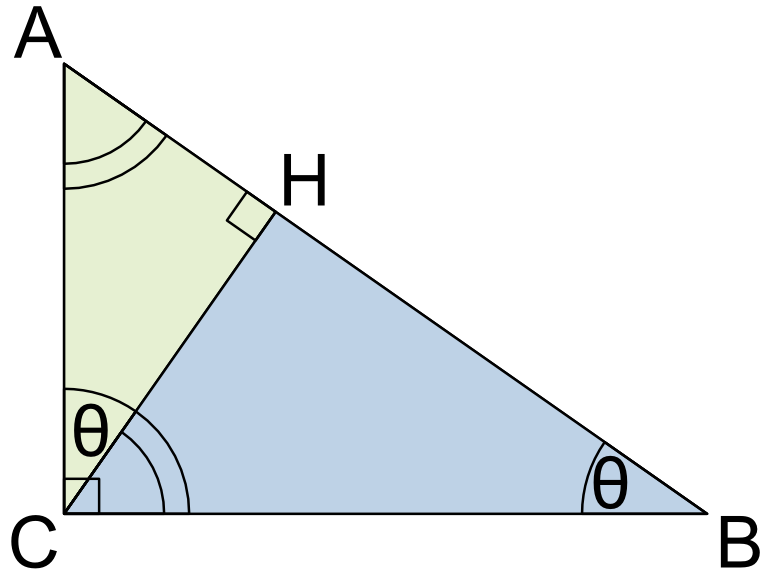
\includegraphics[width=0.3\textwidth]{figures/Pythagoras.png}
	\caption{Similar triangles used in the proof of the Pythagorean theorem.}
	\label{fig:Pythagoras}
\end{figure}

The new triangle $ACH$ is similar to triangle $ABC$, because they both have a right angle (by definition of the altitude), and they share the angle at $A$, meaning that the third angle will be the same in both triangles as well, marked as $\theta$ in Figure~\ref{fig:Pythagoras}. By a similar reasoning, the triangle $CBH$ is also similar to $ABC$. 

Similarity of the triangles leads to the equality of ratios of corresponding sides:
\begin{equation}
    \frac{BC}{AB}=\frac{BH}{BC} \text{ and } \frac{AC}{AB}=\frac{AH}{AC}.
\end{equation}
The first result equates $\cos \theta$ and the second result equates $\sin \theta$.

These ratios can be written as:
\begin{equation}
    {BC}^{2}={AB}\times {BH} \text{ and }{AC}^{2}={AB}\times {AH}.
\end{equation}
Summing these two equalities, we obtain:
\begin{equation}
    {BC}^{2}+{AC}^{2}={AB}\times {BH}+{AB}\times {AH}={AB}\times({AH}+{BH})={AB}^{2} ,
\end{equation}
which, tidying up, is the Pythagorean theorem:
\begin{equation}
    {BC}^{2}+{AC}^{2}={AB}^{2}.
\end{equation}
\end{proof}
%
\end{appendices}
%--------------------------------------------------------------------------------------------------
%
% BACK MATTER
%--------------------------------------------------------------------------------------------------
%
\backmatter
%
% References used in the thesis
\printreferences
% 
% Author's bibliography 
%--------------------------------------------------------------------------------------------------
% 
\chapter{Bibliography}
%--------------------------------------------------------------------------------------------------
% Enclose with refsection and use \nocite{*}, if you need to list publications not referenced in 
% the thesis:
\begin{refsection}
\nocite{*}

\section*{Publications Related to the Thesis}

All publications related to the thesis should be referenced in the text.

\defbibheading{subbibliography}{\subsection*{Journal Articles}}
\printbibliography[heading=subbibliography,env=nolabelbib,sorting=nty,keyword=myarticle]

\defbibheading{subbibliography}{\subsection*{Conference Paper}}
\printbibliography[heading=subbibliography,env=nolabelbib,sorting=nty,keyword=myconf]

\section*{Other Publications (optional)}

\dots

\end{refsection}
%
% Author's biography
%--------------------------------------------------------------------------------------------------
%
\chapter{Biography}
%--------------------------------------------------------------------------------------------------

Jan Rupnik was born in Ljubljana on 6.12.1982. 
 
Following graduation at the Faculty of Mathematics and Physics, University of Ljubljana, 
with a degree in applied mathematics (Diploma) in 2006, he was employed as a researcher 
at the Artificial Intelligence Laboratory, Jožef Stefan Institute. In 2007 he
enroled in the New Media and E-science doctoral study program at the Jožef Stefan 
International Postgraduate School in Ljubljana, Slovenia.

His research interests include Machine Learning, Data Mining, Data
Fusion, Cross-Lingual Text Mining, Predictive Analytics, Applications of Data Mining
in different domains. Most of his research work is connected to the development of
statistical methods that enable cross-modal data integration, with focus on
scalability. 

Jan Rupnik has been involved in a number of EU FP7 projects, including
SMART (Statistical Multilingual Analysis For Retrieval And Translation), XLIKE (Cross-
lingual Knowledge Extraction), EURIDICE (The Intelligent Cargo Concept in the
European Project) and SOPHOCLES (Self-Organised information PrOcessing,
CriticaLity and Emergence in multilevel Systems).
%
% Index (optional)
\printmyindex
%--------------------------------------------------------------------------------------------------
\end{document}
%--------------------------------------------------------------------------------------------------
%
% MODIFICATION HISTORY
%--------------------------------------------------------------------------------------------------
% Version 1.2: 
%  - Modified the symbols and abbreviations example to adjust the vertical positioning of the text
% Version 1.1: 
%  - Removed slovene.lbx and slovene-apa.lbx from accompanying files as they are now included in 
%    the latest biblatex version.
%  - Modified the bibliography example to include publications not referenced before.
%  - Modified the references example to show DOI should be used only for articles not yet published. 
%  - Modified the symbols and abbreviations example to accommodate long lines and long lists.
%  - Added pdf bookmarks for Acknowledgments, Abstract and Povzetek. 
%--------------------------------------------------------------------------------------------------
